\documentclass[Deriaz_Traiber_Labo02]{subfiles}


\begin{document}
\chapter{Antenne dipôle}
\section{Objectif}
Le but est de réaliser une antenne qui résonne autour de \SI{2.45}{\giga\hertz}. Le $s_{11}$ à cette fréquence doit être inférieur à \SI{10}{\deci\bel}.


\begin{figure}[H]
\centering
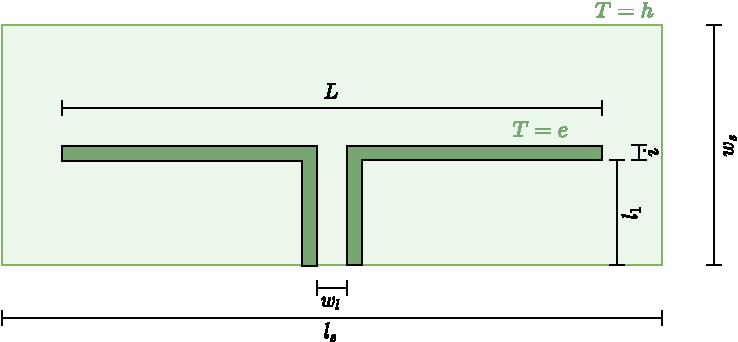
\includegraphics[scale=1,page=1]{../Schemas-crop.pdf}
\caption{Dimensions de l'antenne dipôle}
\end{figure}
\begin{table}[H]
\centering
\begin{tabular}{lll}
\textbf{Variables}\\\hline
$l_1$ & Hauteur du pied\\
$i$ & Épaisseur des brins\\
$L$ & Longueur de l'antenne\\
\textbf{Constantes} & & \textbf{Valeur}\\\hline
$w_l$ & Espacement entre les brins\\
$w_s$ & Largeur du PCB & \SI{30}{\milli\meter}\\
$l_s$ & Longueur du PCB & \SI{80}{\milli\meter}\\
$h$ & Épaisseur du PCB & \SI{1.6}{\milli\meter}\\
$e$ & Épaisseur de cuivre & \SI{35}{\micro\meter}
\end{tabular}
\caption{Liste des dimensions}
\end{table}


\section{FR-4}
La longueur des brins est donnée par l'équation \ref{eq_dipole_longueur}
\begin{equation}
\boxed{L = \dfrac{\lambda}{2\sqrt{\epsilon_r}} = \dfrac{c}{2 f \sqrt{\epsilon_r}}} \Rightarrow \boxed{L = \dfrac{3e8}{2\cdot2.45e9\sqrt{4.3}}=\SI{29.5}{\milli\meter}}
\label{eq_dipole_longueur}
\end{equation}
La dimension du pied est donnée par
\begin{equation}
\boxed{l_1=\frac{\lambda}{8}=\frac{c}{8f}=\SI{15.3}{\milli\meter}}
\end{equation}
La largeur des brins ($i$) a été fixée à \SI{0.8}{\milli\meter} pour le moment.
\subsection{Itérations}
\subsubsection{Premières itérations}

Afin de ce familiariser avec le dimensionnement de l'antenne planaire, la méthode utilisé consiste à modifier un seul des paramètres jusqu'à obtenir le résultat le plus proche possible des performances souhaitées puis de réaliser le même démarche pour un second paramètre et ainsi de suite pour les autre paramètre.


\figc{1}{ant1_FR4_1}{Dimensionnement de l'antenne en ne variant que $L$}

Une fois la meilleur valeur de $L$ déterminée, il est ensuite nécessaire d'améliorer les performances de l'antenne en variant uniquement la longueur $L_2$ et en gardant la longueur $L$ déterminée à l'étape précédente.
\figc{1}{ant1_FR4_2}{Dimensionnement de l'antenne en variant que $l_1$}

\subsection{Balayage des paramètres variables}

\figc{1}{bipol_param_sweep_fr4}{Balayage de paramétrique de l'antenne bipolaire avec substrat FR4}

\figc{1}{bipol_param_norm_sweep_fr4}{Variation normalisée des performances}

\begin{table}[H]
\centering
\begin{tabular}{|l|c|cc|cc|cc|c|}\hline
	Var 		   	& ID  &  $S_{11}$ \si{[\decibel]} &  $dS_{11}$ \si{[\percent]}   &  $F_c$ \si{[\giga\hertz]} &   $dF_c$ \si{[\percent]}  & $BW$\si{[\mega\hertz]} &   $dBW$ \si{[\percent]}  \\ \hline\hline
	
	i - 10\% 	& 1   &  -32.19   &   0.29715   & 2.452   &  -0.80906  &   260   &   -1.5152\\
    i - 1\%     & 2   &  -30.763  &    -4.1498  &   2.68  &     8.4142 &    292  &     10.606\\ 
    	i + 0\%       & 3   &  -32.095  &          0  &  2.472  &          0 &    264  &        0\\
    i + 1\%     & 4   &  -32.326  &    0.72114  &  2.428  &    -1.7799 &    260  &    -1.5152\\
    i + 10\%    & 5   &  -33.418  &     4.1218  &  2.256  &    -8.7379 &    236  &    -10.606\\\hline
    l1 - 10\%   & 6   &  -30.849  &    -3.8817  &  2.448  &   -0.97087 &    260  &    -1.5152\\
    l1 - 1\%    & 7   &  -32.077  &  -0.056551  &  2.452  &   -0.80906 &    260  &    -1.5152\\
    l1 + 1\%    & 8   &  -32.302  &    0.64708  &  2.452  &   -0.80906 &    260  &    -1.5152\\
    l1 + 10\%   & 9   &  -33.309  &     3.7842  &  2.452  &   -0.80906 &    264  &          0\\\hline
    l2 - 10\%   & 10  &  -32.641  &     1.7011  &  2.452  &   -0.80906 &    260  &    -1.5152\\
    l2 - 1\%    & 11  &  -32.235  &    0.43667  &  2.452  &   -0.80906 &    260  &    -1.5152\\
    l2 + 1\%    & 12  &  -31.888  &   -0.64415  &  2.448  &   -0.97087 &    256  &    -3.0303\\
    l2 + 10\%   & 13  &  -32.139  &    0.13769  &  2.452  &   -0.80906 &    260  &    -1.5152\\\hline
    ls - 10\%   & 14  &  -31.693  &    -1.2519  &  2.452  &   -0.80906 &    260  &    -1.5152\\
    ls - 1\%    & 15  &  -32.207  &    0.34869  &  2.452  &   -0.80906 &    260  &    -1.5152\\
    ls + 1\%    & 16  &  -32.229  &    0.41726  &  2.452  &   -0.80906 &    260  &    -1.5152\\
    ls + 10\%   & 17  &  -32.621  &     1.6405  &  2.452  &   -0.80906 &    264  &          0\\\hline
    ws - 10\%   & 18  &  -32.83   &      2.29   & 2.456   &  -0.64725  &   260   &   -1.5152\\
    ws - 1\%    & 19  &  -32.329  &    0.73046  &  2.452  &   -0.80906 &    260  &    -1.5152\\
    ws + 1\%    & 20  &  -32.117  &   0.068609  &  2.448  &   -0.97087 &    260  &    -1.5152\\
    ws + 10\%   & 21  &  -31.623  &      -1.47  &  2.448  &   -0.97087 &    260  &    -1.5152\\\hline
\end{tabular}
\caption{Table de la variation des performances de l'antenne - FR4}
\label{tab:param-sweep-fr4}
\end{table}

\section{Céramique}

\subsection{Balayage des paramètres variables}

\figc{1}{bipol_param_sweep_alumina}{Balayage de paramétrique de l'antenne bipolaire avec substrat en céramique}

\figc{1}{bipol_param_norm_sweep_alumina}{Variation normalisée des performances}

\subsection{Rayonnement de l'antenne}
\subsubsection{Directivité}
\figc{1}{bipol_farfield_dir_fr4}{Directivité de l'antenne - Céramique}

\begin{table}[H]
\centering
\begin{tabular}{l c}\hline
Type				& Farfield\\
Approximation	& enable($kR>>1$)\\
Component		& Abs\\
Output			& Directivity\\
Frequency		& \SI{2.45}{\giga\hertz}\\
Rad. Effic.		& \SI{-0.01015}{\decibel i}\\
Tot. Effic.		& \SI{-0.01256}{\decibel i}\\
Dir.				& \SI{2.421}{\decibel i}\\\hline
\end{tabular}
\end{table}

\subsubsection{Gain IEEE}
\figc{1}{bipol_farfield_gain_ieee_fr4}{Gain IEEE de l'antenne Céramique}

\begin{table}[H]
\centering
\begin{tabular}{l c}\hline
Type				& Farfield\\
Approximation	& enable($kR>>1$)\\
Component		& Abs\\
Output			& Gain\\
Frequency		& \SI{2.45}{\giga\hertz}\\
Rad. Effic.		& \SI{-0.01015}{\decibel i}\\
Tot. Effic.		& \SI{-0.01256}{\decibel i}\\
Gain				& \SI{2.411}{\decibel i}\\\hline
\end{tabular}
\end{table}

\subsubsection{Gain Realized}
\figc{1}{bipol_farfield_gain_rzd_fr4}{Gain Realized de l'antenne Céramique}

\begin{table}[H]
\centering
\begin{tabular}{l c}\hline
Type				& Farfield\\
Approximation	& enable($kR>>1$)\\
Component		& Abs\\
Output			& Realized Gain\\
Frequency		& \SI{2.45}{\giga\hertz}\\
Rad. Effic.		& \SI{-0.01015}{\decibel i}\\
Tot. Effic.		& \SI{-0.01256}{\decibel i}\\
Rlzd. Gain		& \SI{2.408}{\decibel i}\\\hline
\end{tabular}
\end{table}


\begin{table}[H]
\centering
\begin{tabular}{|l|c|cc|cc|cc|c|}\hline
	Var 		   	& ID  &  $S_{11}$ \si{[\decibel]} &  $dS_{11}$ \si{[\percent]}   &  $F_c$ \si{[\giga\hertz]} &   $dF_c$ \si{[\percent]}  & $BW$\si{[\mega\hertz]} &   $dBW$ \si{[\percent]}\\ \hline\hline
       i - 10\%    &  1  &  -16.683  &     -0.84429  &  2.444   &   -0.1634  &   252  & -3.0769\\
    i - 1\%     &  2  &  -16.431  &      -2.3437  &   2.66   &    8.6601  &   284  &  9.2308\\
    + 0\%       &  3  &  -16.825  &            0  &  2.448   &         0  &   260  &       0\\
    i + 1\%     &  4  &  -16.836  &     0.066212  &  2.448   &         0  &   260  &       0\\
    i + 10\%    &  5  &  -16.849  &      0.14586  &  2.448   &         0  &   260  &       0\\\hline
    l1 - 10\%   &  6  &  -16.994  &       1.0042  &  2.452   &    0.1634  &   264  &  1.5385\\
    l1 - 1\%    &  7  &  -16.954  &      0.76524  &  2.456   &    0.3268  &   260  &       0\\
    l1 + 1\%    &  8  &  -16.846  &      0.12802  &  2.452   &    0.1634  &   256  & -1.5385\\
    l1 + 10\%   &  9  &  -16.825  &  -0.00029718  &  2.448   &         0  &   260  &       0\\\hline
    l2 - 10\%   & 10  &  -16.726  &     -0.58812  &  2.444   &   -0.1634  &   260  &       0\\
    l2 - 1\%    & 11  &  -16.805  &     -0.11929  &  2.468   &   0.81699  &   260  &       0\\
    l2 + 1\%    & 12  &  -16.859  &      0.20505  &  2.432   &  -0.65359  &   256  & -1.5385\\
    l2 + 10\%   & 13  &  -17.083  &       1.5331  &  2.272   &   -7.1895  &   232  & -10.769\\\hline
    ls - 10\%   & 14  &  -16.195  &       -3.743  &  2.448   &         0  &   248  & -4.6154\\
    ls - 1\%    & 15  &  -16.781  &     -0.25861  &  2.448   &         0  &   260  &       0\\
    ls + 1\%    & 16  &   -16.89  &      0.38859  &  2.448   &         0  &   260  &       0\\
    ls + 10\%   & 17  &  -17.307  &        2.864  &  2.452   &    0.1634  &   268  &  3.0769\\\hline
    ws - 10\%   & 18  &  -17.005  &       1.0731  &  2.452   &    0.1634  &   260  &       0\\
    ws - 1\%    & 19  &  -16.853  &      0.16719  &  2.448   &         0  &   260  &       0\\
    ws + 1\%    & 20  &   -16.82  &      -0.0274  &  2.448   &         0  &   260  &       0\\
    ws + 10\%   & 21  &  -16.682  &     -0.85065  &  2.448   &         0  &   256  & -1.5385\\\hline
\end{tabular}
\caption{Table de la variation des performances de l'antenne - Céramique}
\label{tab:param-sweep-alumina}
\end{table}

\subsection{Rayonnement de l'antenne}
\subsubsection{Directivité}
\figc{1}{bipol_farfield_dir_alumin}{Directivité de l'antenne - Céramique}

\begin{table}[H]
\centering
\begin{tabular}{l c}\hline
Type				& Farfield\\
Approximation	& enable($kR>>1$)\\
Component		& Abs\\
Output			& Directivity\\
Frequency		& \SI{2.45}{\giga\hertz}\\
Rad. Effic.		& \SI{-0.01119}{\decibel i}\\
Tot. Effic.		& \SI{-0.09294}{\decibel i}\\
Dir.				& \SI{2.820}{\decibel i}\\\hline
\end{tabular}
\end{table}

\subsubsection{Gain IEEE}
\figc{1}{bipol_farfield_gain_ieee_alumin}{Gain IEEE de l'antenne Céramique}

\begin{table}[H]
\centering
\begin{tabular}{l c}\hline
Type				& Farfield\\
Approximation	& enable($kR>>1$)\\
Component		& Abs\\
Output			& Gain\\
Frequency		& \SI{2.45}{\giga\hertz}\\
Rad. Effic.		& \SI{-0.01119}{\decibel i}\\
Tot. Effic.		& \SI{-0.09294}{\decibel i}\\
Gain				& \SI{2.809}{\decibel i}\\\hline
\end{tabular}
\end{table}

\subsubsection{Gain Realized}
\figc{1}{bipol_farfield_gain_rzd_alumin}{Gain Realized de l'antenne Céramique}

\begin{table}[H]
\centering
\begin{tabular}{l c}\hline
Type				& Farfield\\
Approximation	& enable($kR>>1$)\\
Component		& Abs\\
Output			& Realized Gain\\
Frequency		& \SI{2.45}{\giga\hertz}\\
Rad. Effic.		& \SI{-0.01119}{\decibel i}\\
Tot. Effic.		& \SI{-0.09294}{\decibel i}\\
Rlzd. Gain	 	& \SI{2.727}{\decibel i}\\\hline
\end{tabular}
\end{table}







\end{document}